\documentclass[letterpaper,12pt,oneside]{article}
\usepackage[top=1in, left=1.25in, right=1.25in, bottom=1in]{geometry}

\usepackage[T1]{fontenc}
\usepackage[utf8]{inputenc}
\usepackage[english]{babel}
\usepackage{caption, subcaption}
\usepackage{graphicx}
\usepackage{array}
\usepackage{booktabs}
\usepackage{amsmath,amssymb}
\usepackage{tikz}
\usepackage{imakeidx}
\usepackage{hyperref}
\usepackage{biblatex}
\addbibresource{bib/protocolo.bib}

\graphicspath{{./}{./figs/}}
\usepackage{setspace}

\hypersetup{
    colorlinks=true,
    linkcolor=black,
    citecolor=blue!70!black,
    urlcolor=blue!70!black
}

\begin{document}

% =========================================================================
% TITLE PAGE
% =========================================================================
\begin{titlepage}
    \setlength{\parindent}{0pt} \setlength{\parskip}{0pt}

    \begin{center}
        \vfill 
        
        \begin{minipage}{\textwidth}
            \begin{center}
                
\includegraphics[width=4.2cm]{UNAM_LOGO2.png}    
            \end{center}     
            \begin{center}
                \Huge\textbf{Universidad Nacional Autónoma de México}
            \end{center} 
        \end{minipage}
            
        \vfill
        
        \begin{minipage}{0.85\textwidth}
            \begin{center}
                \Large School of Engineering \\[0.2cm]
                \large Computer Engineering
            \end{center}
        \end{minipage}
        
        \begin{center}
            \vfill
            {\Large \textbf{Compilers (Group 5)}} \\[0.3cm]
            {\normalsize Professor: M.I. René Adrián Dávila Pérez}
        \end{center}
        
        \begin{center}
            \vspace*{0.8cm}
            {\LARGE \textbf{PROJECT REPORT: LEXICAL ANALYZER (LEXER)}}\\[0.3cm]
            {\large Architecture package: \texttt{unam.fi.compilers.g5.05}}\\
            \vspace*{0.8cm}
            
            \begin{center}
                \textbf{TEAM 05 MEMBERS:} \\[0.25cm]
                319088058 \textit{(Documentation)} \\
                321634421 \textit{(Project Manager)} \\
                321037530 \textit{(Software Developer)} \\
                424490412 \textit{(State Machine Design)} \\
                321009298 \textit{(General Presenter)}
            \end{center}
            
            \bigskip
            
            \textbf{Group:} 5 \\
            \textbf{Semester:} 2027-1
        \end{center}
        
        \vfill
        
        \begin{center}
            {Ciudad Universitaria, Mexico City. October 2026}\\
            {\footnotesize Public repository: \url{https://github.com/alanvilchisssss/Compilers_Repository}}
        \end{center}
        \cleardoublepage
    \end{center}
\end{titlepage}

\tableofcontents
\clearpage

% =========================================================================
% SECTION 1: INTRODUCTION
% =========================================================================
\section{Introduction}

\subsection{Problem statement}
A compiler translates programs written in a high-level language into low-level code that a machine can run. The first step of this process is the lexical analysis. In this step, the program reads the source code as a long list of characters and turns it into a list of small units with meaning, called \textit{tokens}.

In this project we had to design and build a lexical analyzer (\textit{lexer}) for a small part of a C/C++ style language. We were not allowed to use automatic tools like FLEX. The lexer has to read text typed in the console and also plain text files. It must classify each token in the correct category (keywords, including the token \texttt{print}, identifiers, constants, operators and punctuation). It also has to ignore single-line and multi-line comments. To check that it works, we had to run a test with at least 40 tokens. Finally, we had to prepare the theory for the next phase, the syntax analysis. For this, we wrote a Context-Free Grammar (CFG) and applied the \textit{Left Factoring} technique to it.

\subsection{Motivation}
Keeping the lexical analysis separate from the syntax analysis is a basic idea in compiler design~\cite{10.5555/576122}. If the parser had to read the source code character by character, the grammar would be much harder to design and the program would be slower. When the lexer works as a separate part:
\begin{itemize}
    \item The parser is easier to design, because the grammar works with tokens and not with single characters.
    \item The program runs faster, because pattern matching with regular expressions is very efficient.
    \item Details like spaces, tabs and comments are handled in one place, so they do not appear in the syntax rules.
\end{itemize}

\subsection{Objectives}
\textbf{General objective:} \\
To build a modular lexical analyzer inside the package \texttt{unam.fi.compilers.g5.05}. It must recognize, classify and count the tokens of source code that comes from the console or from a text file. We test it with a case of 40 tokens, and we prepare the step to syntax analysis with a CFG that uses left factoring.

\textbf{Specific objectives:}
\begin{itemize}
    \item Add two ways to read the input: text typed in the console and text files with the \texttt{.txt} extension.
    \item Write regular expressions to find keywords (\texttt{keyword}), identifiers (\texttt{identifier}), operators (\texttt{operator}), numbers and text literals (\texttt{constant}) and delimiters (\texttt{punctuation}).
    \item Remove single-line comments (\texttt{//...}) and block comments (\texttt{/*...*/}) without changing the valid tokens.
    \item Propose a Context-Free Grammar for some statements of the language and apply left factoring to remove the problem of common prefixes.
\end{itemize}

% =========================================================================
% SECTION 2: THEORETICAL FRAMEWORK
% =========================================================================
\section{Theoretical Framework}

Lexical analysis and syntax analysis are based on formal languages and automata theory~\cite{10.5555/576122}.

\subsection{Tokens, Patterns and Lexemes}
There are three important ideas in the lexical analysis:
\begin{itemize}
    \item \textbf{Token:} A pair made of a name that represents a grammar unit (for example \texttt{keyword} or \texttt{identifier}) and an optional attribute.
    \item \textbf{Lexeme:} The real group of characters in the source code that matches the pattern of a token (for example \texttt{printf}, \texttt{10}, \texttt{<=}).
    \item \textbf{Pattern:} A formal rule, usually a regular expression, that says which characters a lexeme needs to have to belong to a token.
\end{itemize}

\subsection{Context-Free Grammars (CFG)}
A Context-Free Grammar is defined as a 4-tuple $G = (V, \Sigma, R, S)$, where:
\begin{itemize}
    \item $V$ is a finite set of non-terminal symbols (syntax variables).
    \item $\Sigma$ is a finite set of terminal symbols. It has no elements in common with $V$ ($\Sigma \cap V = \emptyset$). These symbols are the tokens that the lexer gives.
    \item $R$ is a finite set of production rules with the form $A \to \alpha$, where $A \in V$ and $\alpha \in (V \cup \Sigma)^*$.
    \item $S \in V$ is the start symbol of the grammar.
\end{itemize}

\subsection{Non-Determinism and Left Factoring}
A top-down predictive parser, like an $LL(1)$ parser, has to choose which production to use by looking only at the next input token (\textit{lookahead}). Sometimes two or more productions of the same non-terminal start with the same symbols (a common prefix). In that case, the parser cannot know which rule is the correct one. It would need to go back and try again (\textit{backtracking}). This problem is called non-determinism.

\textbf{Left Factoring} solves this problem. It changes the grammar by taking out the common prefix. For example, if we have a production like this:
\begin{equation}
    A \to \alpha \beta_1 \mid \alpha \beta_2 \mid \dots \mid \alpha \beta_n \mid \gamma
\end{equation}
where $\alpha \neq \varepsilon$ is the longest common prefix and $\gamma$ represents the productions that do not start with $\alpha$, then we add a new non-terminal $A'$ and we get:
\begin{align}
    A &\to \alpha A' \mid \gamma \\
    A' &\to \beta_1 \mid \beta_2 \mid \dots \mid \beta_n
\end{align}

\subsubsection{Applying Left Factoring to the Example Statements}
We take the two test statements from the project instructions:
\begin{center}
    \texttt{int a = 10;} \quad and \quad \texttt{printf("This is an example");}
\end{center}

First we define a base grammar. In this grammar, declarations and function calls have alternatives that share the same prefix:
\begin{align}
    S &\to \text{Decl} \mid \text{Call} \\
    \text{Decl} &\to \text{type} \ \mathbf{id} \ \mathbf{;} \;\Big|\; \text{type} \ \mathbf{id} \ \mathbf{=} \ \text{Expr} \ \mathbf{;} \label{eq:decl_orig} \\
    \text{Call} &\to \mathbf{printf} \ \mathbf{(} \ \mathbf{string} \ \mathbf{)} \ \mathbf{;} \;\Big|\; \mathbf{printf} \ \mathbf{(} \ \mathbf{string} \ \mathbf{,} \ \text{Arg} \ \mathbf{)} \ \mathbf{;} \label{eq:call_orig}
\end{align}
The other variables produce the lexical units that the lexer recognizes:
\begin{align}
    \text{type} &\to \mathbf{int} \mid \mathbf{float} \mid \mathbf{char} \mid \mathbf{void} \\
    \text{Expr} &\to \mathbf{id} \mid \mathbf{constant} \\
    \text{Arg} &\to \mathbf{id} \mid \text{Expr}
\end{align}

In rule~(\ref{eq:decl_orig}), both alternatives start with the common prefix $\alpha = \text{type} \ \mathbf{id}$. After left factoring we get:
\begin{align}
    \mathbf{Decl} &\to \text{type} \ \mathbf{id} \ \mathbf{Decl'} \\
    \mathbf{Decl'} &\to \mathbf{;} \;\Big|\; \mathbf{=} \ \text{Expr} \ \mathbf{;}
\end{align}

In rule~(\ref{eq:call_orig}), both alternatives start with the prefix $\alpha = \mathbf{printf} \ \mathbf{(} \ \mathbf{string}$. We apply the same change:
\begin{align}
    \mathbf{Call} &\to \mathbf{printf} \ \mathbf{(} \ \mathbf{string} \ \mathbf{Call'} \\
    \mathbf{Call'} &\to \mathbf{)} \ \mathbf{;} \;\Big|\; \mathbf{,} \ \text{Arg} \ \mathbf{)} \ \mathbf{;}
\end{align}

Now the productions do not have common prefixes. The parser does not choose a rule too early, so it does not need backtracking. This makes it easier to build a top-down predictive parser.

% =========================================================================
% SECTION 3: DEVELOPMENT
% =========================================================================
\section{Development}

Following the delivery rules, we organized the solution in the package \texttt{unam.fi.compilers.g5.05}. We managed the work in a public GitHub repository. Each member of the team had one main role: project management, development, state analysis, presentation or documentation.

\subsection{How the Implementation Works}
The system does not use any automatic lexer generator. It has two main functions:

\begin{enumerate}
    \item \textbf{Input module (\texttt{cadena\_input}):} \\
    The user chooses where the text comes from. With the direct option, the program reads the text from the terminal. With the file option, the program asks for the name of a file in the local folder. It checks that the file has the \texttt{.txt} extension. If the file does not exist, the program catches the error and does not crash.
    
    \item \textbf{Token recognition module (\texttt{identificar\_tokens}):} \\
    This module uses regular expressions and works in two steps:
    \begin{itemize}
        \item \textit{Splitting with one pattern:} We do not split the text by spaces, because that would break text constants and operators with two characters. Instead, we wrote one big regular expression where the order of the parts matters. This pattern looks first for block and line comments, then complete strings between quotes, real and integer numbers, identifiers, two-character operators (\texttt{==}, \texttt{!=}, \texttt{<=}, \texttt{>=}), one-character operators, punctuation and, at the end, any other symbol.
        \item \textit{Filtering and classification:} While the program goes through the elements it found, it skips the comments, so they are not counted as tokens. After that, it compares each lexeme with the pattern of each category: \texttt{keyword}, \texttt{identifier}, \texttt{operator}, \texttt{constant} and \texttt{punctuation}. The tokens are saved in lists, one for each category, and the program also keeps the total count.
    \end{itemize}
\end{enumerate}

\subsection{Tests}
We used two test cases to check the analyzer:

\begin{itemize}
    \item \textbf{Basic statement test (interactive mode):} \\
    \textbf{Input:} The example statement from the instructions: \texttt{printf("This is an example");}. \\
    \textbf{Expected output:} One keyword (\texttt{printf}), one string constant (\texttt{"This is an example"}) and three punctuation symbols (\texttt{(}, \texttt{)}, \texttt{;}). This gives a total of 5 tokens.
    
    \item \textbf{Full source code test (\texttt{prueba\_40\_tokens.txt}):} \\
    \textbf{Input:} A file with a comment at the top and a block of C/C++ code. The code has declarations with initial values (\texttt{int a = 10;}, \texttt{float b = 30.5;}), a condition (\texttt{if (a <= b)}), calls to print functions (\texttt{print("ok");} and \texttt{printf("This is an example");}), a return (\texttt{return a;}), an arithmetic assignment (\texttt{x = a + b;}) and a simple declaration (\texttt{char c;}). \\
    \textbf{Expected output:} The program ignores the first comment and classifies exactly 40 tokens in the five categories.
\end{itemize}

% =========================================================================
% SECTION 4: RESULTS
% =========================================================================
\section{Results}

This section shows the evidence of the tests we ran with the lexical analyzer.

\begin{figure}[htbp]
    \centering
    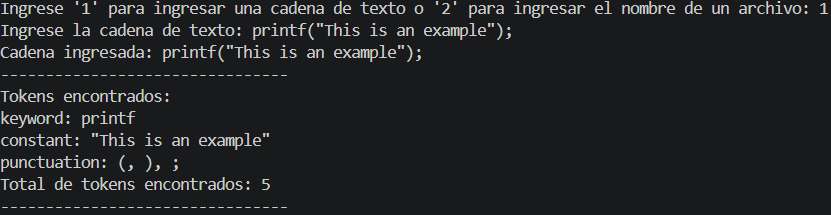
\includegraphics[width=0.85\textwidth]{captura1.png}
    \caption{Interactive run of the analyzer with the example statement \texttt{printf("This is an example");}.}
    \label{fig:ejecucion_consola}
\end{figure}

Figure~\ref{fig:ejecucion_consola} shows the program running from the menu with the direct text option. The string with spaces stays complete. The program classifies \texttt{printf} as a keyword, the text as a constant and the other symbols as punctuation. The result is 5 tokens.

\begin{figure}[htbp]
    \centering
    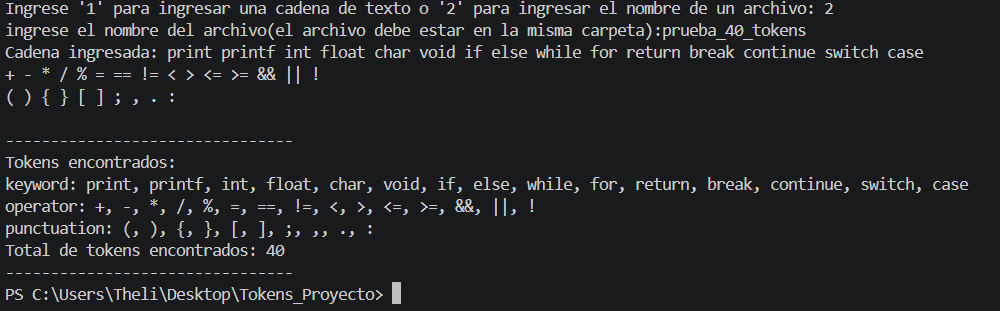
\includegraphics[width=0.85\textwidth]{captura2.png}
    \caption{Processing of the file \texttt{prueba\_40\_tokens.txt} and the total number of tokens found.}
    \label{fig:resultado_40_tokens}
\end{figure}

Figure~\ref{fig:resultado_40_tokens} shows how the program reads the file \texttt{prueba\_40\_tokens.txt}. The analyzer ignored the first comment and processed the rest of the code. It recognized the required keyword (\texttt{print}), the variable names, the two-character relational operator (\texttt{<=}), the arithmetic operators, the integer and real numbers, the strings and the delimiters. Table~\ref{tab:resumen_tokens} shows how many tokens we got in each category.

\begin{table}[htbp]
\centering
\caption{Number of tokens in each category for the 40-token test.}
\label{tab:resumen_tokens}
\begin{tabular}{lcp{8.5cm}}
\toprule
\textbf{Category} & \textbf{Total} & \textbf{Lexemes found} \\
\midrule
\texttt{keyword} & 7 & \texttt{int}, \texttt{float}, \texttt{if}, \texttt{print}, \texttt{return}, \texttt{printf}, \texttt{char} \\
\texttt{identifier} & 9 & \texttt{a}, \texttt{b}, \texttt{a}, \texttt{b}, \texttt{a}, \texttt{x}, \texttt{a}, \texttt{b}, \texttt{c} \\
\texttt{operator} & 5 & \texttt{=}, \texttt{=}, \texttt{<=}, \texttt{=}, \texttt{+} \\
\texttt{constant} & 4 & \texttt{10}, \texttt{30.5}, \texttt{"ok"}, \texttt{"This is an example"} \\
\texttt{punctuation} & 15 & \texttt{;}, \texttt{;}, \texttt{(}, \texttt{)}, \texttt{\{}, \texttt{(}, \texttt{)}, \texttt{;}, \texttt{\}}, \texttt{;}, \texttt{(}, \texttt{)}, \texttt{;}, \texttt{;}, \texttt{;} \\
\midrule
\textbf{Total tokens} & \textbf{40} & \textbf{The 40-token requirement is met} \\
\bottomrule
\end{tabular}
\end{table}

% =========================================================================
% SECTION 5: CONCLUSIONS
% =========================================================================
\section{Conclusions}

From the results, we can say the following:

\begin{itemize}
    \item Using one main pattern with a clear order was necessary to solve the classic problem between simple operators (\texttt{=}) and compound operators (\texttt{<=}). Because the program checks the longer patterns first, the relational operators are always read as one single token.
    \item Removing comments and spaces before the classification keeps the useful tokens separate from the rest of the source code. In this way, the parts of the code that are only for the reader do not affect the syntax analysis that comes later.
    \item The full test with real statements showed that the analyzer can tell the difference between identifiers, keywords, numbers and text constants. It also gave the exact count of 40 tokens that the project asked for.
    \item When we applied left factoring to the rules for declarations and function calls, the common prefixes disappeared. This change is needed to avoid backtracking, and it is the first step to build a deterministic predictive parser.
\end{itemize}

\printbibliography

\end{document}